\begin{frame}
    \frametitle{Future Plans}
    \centering
    \begin{tikzpicture}[-, node distance = 3cm, scale=0.8]
        \node[anchor=north](H1){\(H_1\)};
        \node[anchor=north](H1_d1) at (3, 2){.};
        \node[anchor=north](H1_d2) at (3, -2){.};

        \path[->] (H1) edge node {}(H1_d1);
        \path[->] (H1) edge node {}(H1_d2);
        \path (H1_d1) edge [bend left] node {}(H1_d2);
        \path (H1_d1) [dashed] edge node {}(H1_d2);

        \node[anchor=north](H2) at (3.9, 0){\(H_2\)};
        \node[anchor=north](H2_d1) at (6.9, 2){.};
        \node[anchor=north](H2_d2) at (6.9, -2){.};

        \path[->] (H2) edge node {}(H2_d1);
        \path[->] (H2) edge node {}(H2_d2);
        \path(H2_d1) edge [bend left] node {}(H2_d2);

        \node[anchor=north](A) at (7.8, 0){\(A\)};
        \node[anchor=north](A_d1) at (10.8, 2){.};
        \node[anchor=north](A_d2) at (10.8, -2){.};
        
        \path[->] (A) edge node {}(A_d1);
        \path[->] (A) edge node {}(A_d2);
        \path(A_d1) edge [bend left] node {}(A_d2);
    \end{tikzpicture}
\end{frame}


\begin{frame}
    \frametitle{Future Plans}

    \centering
    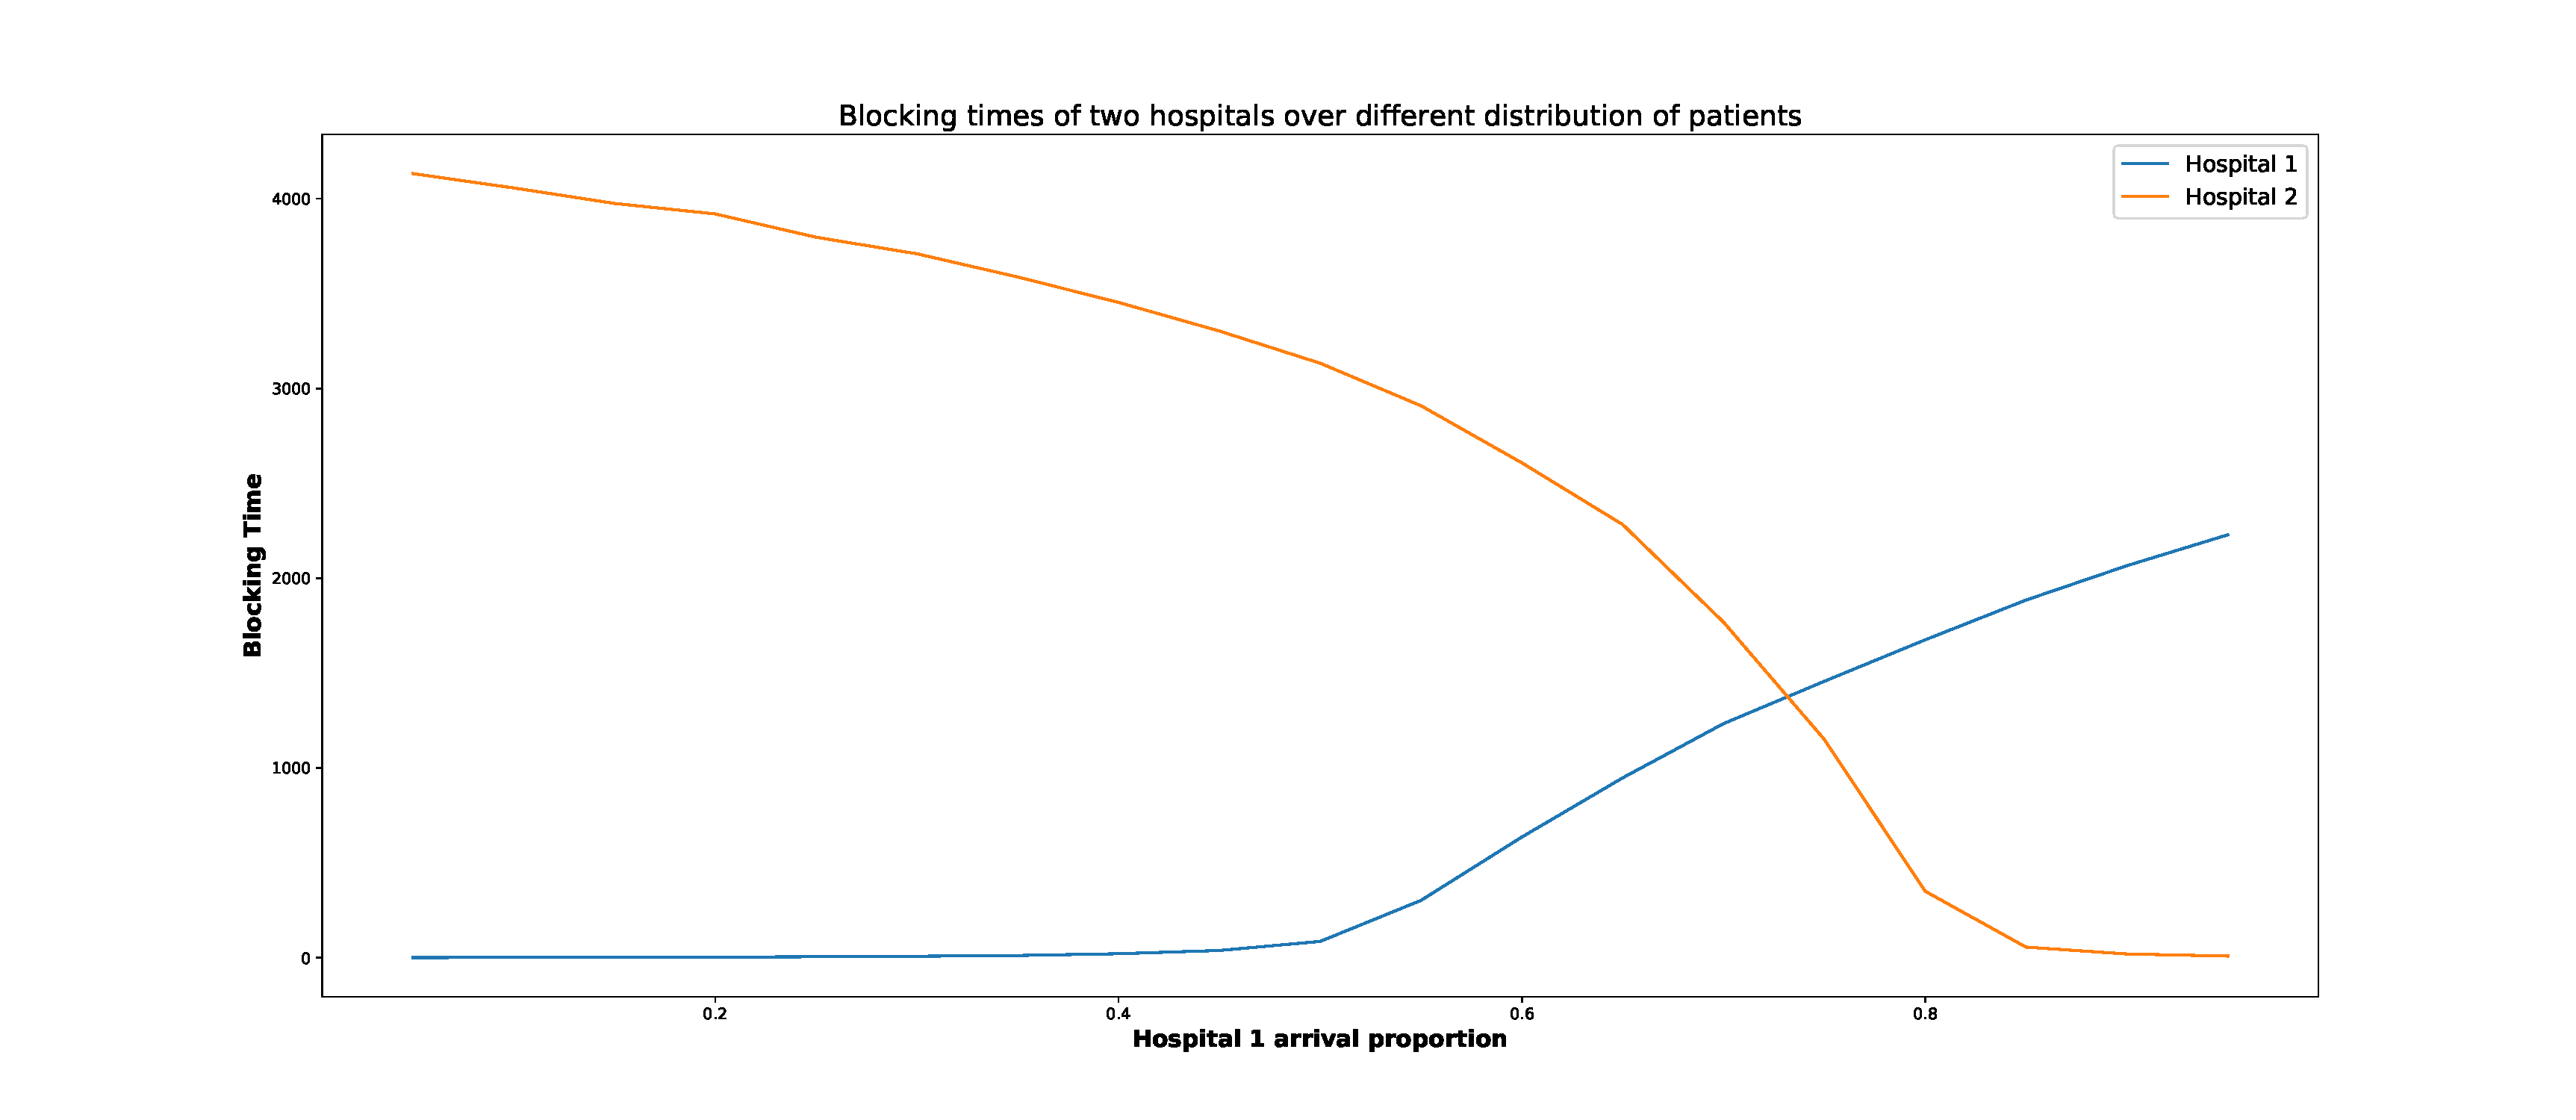
\includegraphics[trim=140 40 150 50, clip, width=\textwidth]{Bin/src/optimal_patient.pdf}
\end{frame}


\begin{frame}
    \frametitle{Future Plans}

    \begin{itemize}
        \item Panayides, M., Knight, V. and Harper, P., 2020. \textit{On a queueing model with two waiting rooms}. 
        \item Panayides, M., Knight, V. and Harper, P., 2020. \textit{A game theoretic model of the ED-EMS interface.}
    \end{itemize}

\end{frame}